% file for pdflatex.exe

% process.tex v1.2 (c) | Copyright 2023 Daniel E. Janusch

% This file is licensed by https://raw.githubusercontent.com/drizzt536/files/main/LICENSE
% and may be copied ONLY IN ITS ENTIRETY under penalty of law.



\documentclass[12pt]{article}
\usepackage{amssymb, latexsym, amsmath, pgfplots, xcolor}
\usepackage[margin=1in]{geometry}

\pgfplotsset{compat=1.18, width=7.5cm}
\definecolor{dimgreen}{RGB}{0, 110, 0}

\pgfmathdeclarefunction{triangleNumber}{1}{
	\pgfmathparse{(#1^2 + #1) / 2}
}

\addtolength{\topmargin}{-0.5in}

\begin{document}


\title{Integrating Functions with Countably Many Jump Discontinuities}
\author{Daniel E. Janusch}
\date{October 6, 2023, 11:13pm MST}

\maketitle

	While applications don't immediately come to attention, the pursuit of knowledge and mathematical literacy
	is enough in itself. Godfrey Harold Hardy (1940), a 20th-century mathematician famously said ``No discovery
	of mine has made, or is likely to make, directly or indirectly, for good or for ill, the least difference
	to~...~the world" (A Mathematician's Apology, 1st ed., p. 49); his work is now used everywhere in essential
	fields like cryptography.

	For the following process to work, the functions are limited to a countable amount of jump discontinuities,
	since if there is an uncountable amount, then by definition, the discontinuities can't be listed out, and
	step~2 won't work. It makes it much easier to assume that there are no discontinuities other than the jump
	discontinuities, but the main essence of the steps should be about the same in that case. This process
	pertains to step functions like $\lfloor x\rfloor$ and $\lceil x\rceil$. The notation used will be as
	follows: $f(x)$ is the full function with the step functions in it and  $g(x)$ is the same function but
	with the step functions removed. For instance, if $f(x)$ is any of $x^2$, $\lfloor x\rfloor^2$,
	$\left\lfloor x^2\right\rfloor$, or $x\lfloor x\rfloor$, then $g(x)=x^2$. Functions like
	$f(x)=\lfloor x\rfloor^2-2\lfloor x\rfloor$ are continuous analogs of discrete functions, so this process
	could introduce a way of integrating discrete functions.

\section*{Step 1: Define a Function to Integrate}

	\indent\indent You can use almost any function you want, but if it is too general steps 3 or 4 might not
	work. Some possible examples for $f(x)$ are $\lfloor x\rfloor$, $\lfloor\sin\pi x\rfloor$,
	$\left\lfloor x^2 - x + 1\right\rfloor$, or $\left\lfloor\frac 1x\right\rfloor$. Usually, if you have
	anything in terms of the ceiling, rounding, or truncating functions, you will want to convert them to the
	floor function with these formulas: $\text{round}(x)=\left\lfloor x+\frac12\right\rfloor$,
	$\lceil x\rceil=-\lfloor-x\rfloor$, and $\text{truncate}(x)=\lfloor|x|\rfloor\text{sgn}(x)$. Sometimes you
	will need to pay attention to the integral boundaries, as for most functions they can be 0 and $x$, but for
	$f(x)=\left\lfloor\frac 1x\right\rfloor$, they should be 1 and $x$. The lower bound should be wherever the
	integral is zero. Don't use a naïve approach like $\int\lfloor x\rfloor\text dx=x\lfloor x\rfloor+c$; while
	taking the derivative of both sides technically does give the same function, it is not correct because it is
	missing $-\frac{\lfloor x\rfloor^2+\lfloor x\rfloor}2$. This is because
	$\displaystyle\lim_{x\to a}\tfrac{\text d\,\lfloor x\rfloor}{\text dx}(a)=0$ for any constant $a$, so
	$\lfloor x\rfloor$ can just be treated as a constant when taking derivatives. Here are a couple graphs.

	\begin{figure}[h]
		\centering
		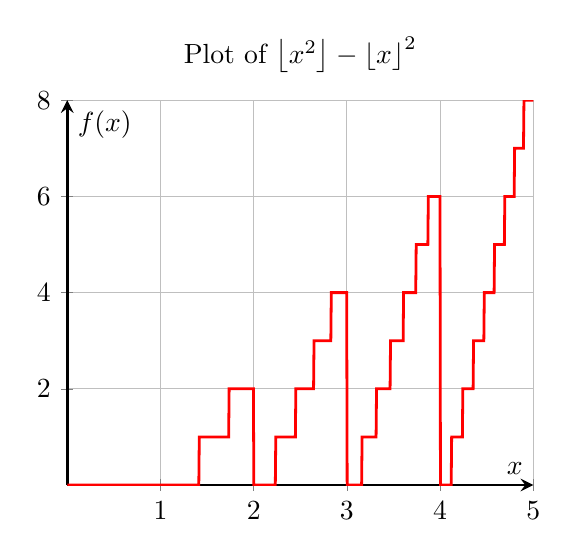
\begin{tikzpicture}
			\begin{axis}[
					xlabel=$x$,
					ylabel=$f(x)$,
					axis lines=middle,
					line width=1.01pt,
					domain=0:5,
					samples=1000,
					grid=both,
					title={Plot of $\left\lfloor x^2 \right\rfloor - \left\lfloor x \right\rfloor^2$},
				]
				\addplot[color=red]{floor(x^2) - floor(x)^2};
			\end{axis}
		\end{tikzpicture}
		\hfill
		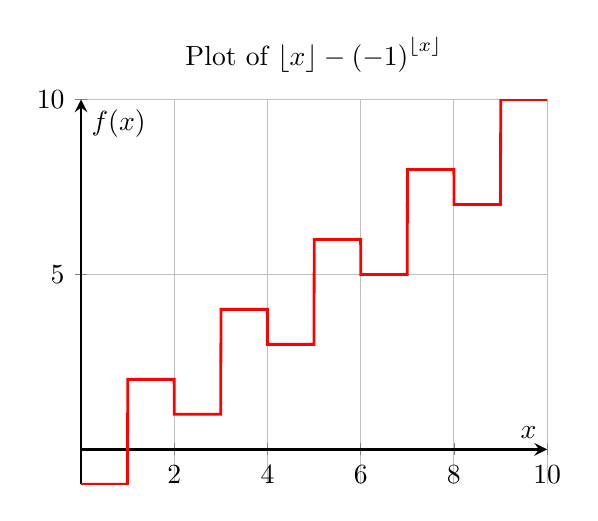
\begin{tikzpicture}
			\begin{axis}[
					xlabel=$x$,
					ylabel=$f(x)$,
					axis lines=middle,
					line width=1.01pt,
					domain=0:10,
					samples=2000,
					grid=both,
					title={Plot of $\lfloor x\rfloor - \left(-1\right)^{\left\lfloor x\right\rfloor}$},
				]
				\addplot[color=red]{floor(x) - (-1)^floor(x)};
			\end{axis}
		\end{tikzpicture}
	\end{figure}

\section*{Step 2: Split at the Jumps and Integrate Separately}

	\indent\indent Since $f(x)$ is not continuous, you need to figure out where the value of $f(x)$ changes,
	or where the $n$th jump discontinuity is. Then you split the integral by these boundaries and integrate
	each interval individually. Sometimes this can be slightly trickier if you have something like
	$f(x)=\sqrt{\lfloor x\rfloor}$ because not all the output values are at integers. You will benefit from
	using a different strategy for periodic functions like $\lfloor\cos x\rfloor$ to take advantage of
	their periodicity. Splitting at jumps is a similar method to how you integrate piecewise functions,
	although in piecewise functions you split the integral at the piece boundaries instead of just at jumps
	(Calculus, Larson \& Edwards, 2010).

	\subsection*{Example 1:}

		\begin{minipage}{0.5\textwidth}
			\begin{align*}
				f(x) & := \left\lfloor\frac x2\right\rfloor\\
				g(x) & = \frac x2\\
				g^{-1}(x) & = 2x\\
				\int_{2n}^{2(n+1)}f(t)\text dt & = \int_{2n}^{2n+2}\left\lfloor\frac t2\right\rfloor\text dt
			\end{align*}
		\end{minipage}
		\hfill
		\begin{minipage}{0.5\textwidth}
			\begin{tikzpicture}
				\begin{axis}[
						xlabel=$x$,
						ylabel=$y$,
						axis lines=middle,
						samples=2000,
						grid=both,
						line width=1.01pt,
						legend pos=inner north east,
						legend style={font=\small},
					]

					\addplot[color=red, domain=0:10]{floor(x/2)};
					\addlegendentry{$f(x)$}

					\addplot[color=blue, domain=0:10]{x/2};
					\addlegendentry{$g(x)$}

					\addplot[color=dimgreen, domain=0:5]{2*x};
					\addlegendentry{$g^{-1}(x)$}
				\end{axis}
			\end{tikzpicture}
		\end{minipage}
		\vspace{0.2em}

		$f(x)$ on this interval will be the same value, so this is just the area of a rectangle.
		Ignore the discontinuities at the endpoints; they don't change the outcome of the integral.

		\begin{align*}
			\int_{2n}^{2n+2}\left\lfloor\frac t2\right\rfloor\text dt
			= \left\lfloor\frac{2n}2\right\rfloor(2n+2-2n)
			= \lfloor n\rfloor\cdot2 = 2n
		\end{align*}

	\subsection*{Example 2:}

		\begin{minipage}{0.5\textwidth}
			\begin{align*}
				f(x) & := \left\lfloor x^2\right\rfloor\\
				g(x) & = x^2\\
				g^{-1}(x) & = \sqrt x\\
			\end{align*}
		\end{minipage}
		\hfill
		\begin{minipage}{0.5\textwidth}
			\begin{tikzpicture}
				\begin{axis}[
						xlabel=$x$,
						ylabel=$y$,
						axis lines=middle,
						samples=1800,
						grid=both,
						line width=1.01pt,
						legend pos=inner north east,
						legend style={font=\small},
					]

					\addplot[color=red, domain=0:5]{floor(x^2)};
					\addlegendentry{$f(x)$}

					\addplot[color=blue, domain=0:5]{x^2};
					\addlegendentry{$g(x)$}

					\addplot[color=dimgreen, domain=0:8]{sqrt(x)};
					\addlegendentry{$g^{-1}(x)$}
				\end{axis}
			\end{tikzpicture}
		\end{minipage}

		doing the same thing as in example 1, we get:

		\begin{align*}
			\int_{\sqrt n}^{\sqrt{n+1}}f(t)\text dt = f(\sqrt n)\left(\sqrt{n+1}-\sqrt n\right)
			= \lfloor x\rfloor\sqrt{1+2x-2\sqrt{x^2+x}}\\
			\text{and in general, }\int_{g^{-1}(n)}^{g^{-1}(n+1)}f(t)\text dt
			=f\left(g^{-1}(n)\right)\left[g^{-1}(n+1)-g^{-1}(n)\right]
		\end{align*}

		This general formula only works if $f(x)$ is constant in between discontinuities. Make sure you
		use the correct area formula for your function. For instance, If you have $f(x)=x\lfloor x\rfloor$
		then use the trapezoid area formula instead.

\section*{Step 3: Find the Sum of Each Partial Integral}

	After you've figured out the closed form of the integral on each interval, you can use the
	additive interval property of integrals, where ``if $f$ is integrable on the three closed
	intervals determined by $a$, $b$, and $c$, then $\int_a^bf(x)dx=\int_a^cf(x)dx+\int_c^bf(x)dx$"
	(Calculus, Larson \& Edwards, 2010, p. 276). Sum up the separate integrals and get the closed
	form on the whole interval. The following summation is impossible for a general $f(x)$, so you
	need to have a specific function for this step.

	\begin{align*}
		\int_{g^{-1}(0)}^{g^{-1}(k)}f(t)\text dt=\sum_{j=1}^{k-1}\int_{g^{-1}(j)}^{g^{-1}(j+1)}f(t)\text dt
	\end{align*}

	Oftentimes you can end up with the general harmonic sequence or a difference of Hurwitz Zeta functions
	as the closed form. Other times the sum can just be impossible to get a closed form for.

	\subsection*{Example:}

		\begin{minipage}{0.5\textwidth}
			\begin{align*}
				f(x) & := \lfloor x\rfloor\\
				g(x) & = x\\
				g^{-1}(x) & = x
			\end{align*}
		\end{minipage}
		\hfill
		\begin{minipage}{0.5\textwidth}
			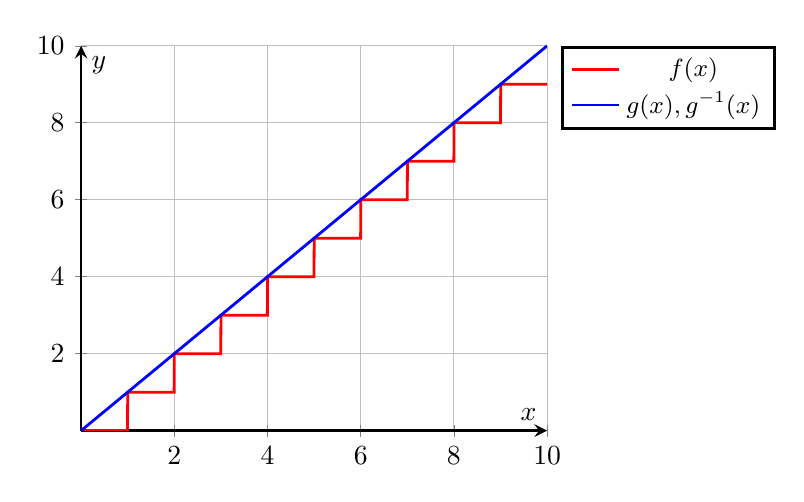
\begin{tikzpicture}
				\begin{axis}[
						xlabel=$x$,
						ylabel=$y$,
						axis lines=middle,
						samples=2000,
						grid=both,
						line width=1.01pt,
						legend pos=outer north east,
						legend style={font=\small},
					]

					\addplot[color=red, domain=0:10]{floor(x)};
					\addlegendentry{$f(x)$}

					\addplot[color=blue, domain=0:10]{x};
					\addlegendentry{$g(x), g^{-1}(x)$}

				\end{axis}
			\end{tikzpicture}
		\end{minipage}

		\begin{align*}
			\int_0^k\lfloor t\rfloor\text dt
			= \sum_{j=0}^{k-1}\int_j^{j+1}\!\lfloor t\rfloor\text dt
			= \sum_{j=1}^{k-1}j[j+1-j]
			= \frac{k^2-k}2
		\end{align*}

\section*{Step 4: Integrate up to $x$}

	To integrate up to $x$, you can once again use the additive interval property of integrals. The first integral (on the right) is from step~3, and the second is similar to in step~2. $g^{-1}(f(x))$ is
	the greatest $x$-value less than $x$ with a jump discontinuity. The formula for the second integral
	is not always correct; use the correct area formula for the section. It is the same process as in
	step~2 but using a subset of the interval.

	\begin{align*}
		\int_{g^{-1}(0)}^xf(t)\text dt & = \int_{g^{-1}(0)}^{g^{-1}(f(x))}f(t)\text dt+\int_{g^{-1}(f(x))}^xf(t)\text dt\\
		\int_{g^{-1}(f(x))}^xf(t)\text dt & = f(x)\!\left[x-g^{-1}(f(x))\right]
	\end{align*}

	\subsection*{Example:}

		\begin{minipage}{0.5\textwidth}
			\begin{align*}
				f(x) & := \lfloor x\rfloor\\
				g(x) & = x\\
				g^{-1}(x) & = x
			\end{align*}
		\end{minipage}
		\hfill
		\begin{minipage}{0.5\textwidth}
			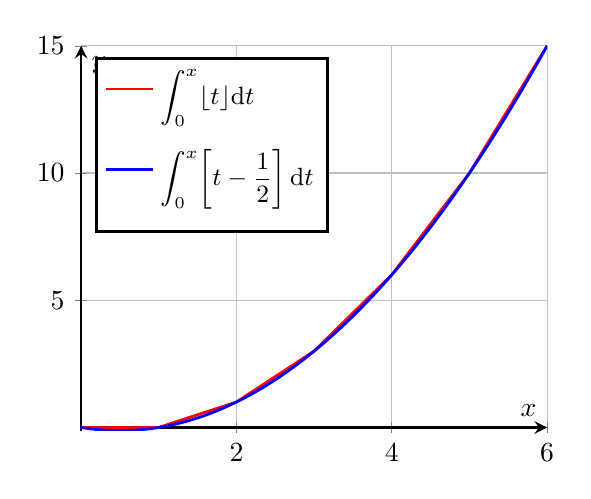
\begin{tikzpicture}
				\begin{axis}[
						xlabel=$x$,
						ylabel=$y$,
						axis lines=middle,
						samples=2000,
						grid=both,
						domain=0:6,
						line width=1.01pt,
						legend pos=north west,
						legend style={font=\small},
						legend cell align=left
					]

					\addplot[color=red]{(floor(x)^2 - floor(x)) / 2 + (x - floor(x)) * floor(x)};
					\addlegendentry{$\displaystyle\int_0^x\lfloor t\rfloor\text dt$}

					\addlegendimage{empty legend}\addlegendentry[]{}
					\addlegendimage{empty legend}\addlegendentry[]{}

					\addplot[color=blue]{(x^2 - x) / 2};
					\addlegendentry{$\displaystyle\int_0^x\!\left[t-\frac12\right]\text dt$}

					\addlegendimage{empty legend}\addlegendentry[]{}
					\addlegendimage{empty legend}\addlegendentry[]{}
				\end{axis}
			\end{tikzpicture}
		\end{minipage}

		\begin{align*}
			\int_{g^{-1}(0)}^xf(t)\text dt
			= \int_0^{\lfloor x\rfloor}\lfloor t\rfloor\text dt+\int_{\lfloor x\rfloor}^x\lfloor t\rfloor\text dt
			= \frac{\lfloor x\rfloor^2-\lfloor x\rfloor}2+(x-\lfloor x\rfloor)\lfloor x\rfloor
		\end{align*}

		Once you have this, you have found the principle indefinite integral. Add the constant of integration
		for the general answer.


\section*{References}
	% I think these are in APA, but I don't really care.
	\begin{itemize}
		\item Hardy, G. H. (1940). A Mathematician's Apology (1st ed.). University of Alberta Mathematical Sciences Society.\\
			\url{https://www.arvindguptatoys.com/arvindgupta/mathsapology-hardy.pdf}\\

		\item Larson, R., & Edwards, B. H. (2010). Calculus (9th ed.). Cengage Learning.\\
			\url{http://teacherpress.ocps.net/cynthiaandrews/files/2013/06/Calculus-9th-Edition-by-Ron-Larson-Bruce-H.-Edwards.pdf}
	\end{itemize}
	\vspace{28em}\\
	This document is licensed under https://raw.githubusercontent.com/drizzt536/files/main/LICENSE
	and may be copied ONLY IN ITS ENTIRETY under penalty of law.

\end{document}
